\documentclass[10pt]{report}
\usepackage{graphicx}
\usepackage{hyperref}
\usepackage[left=1.5cm,right=1.5cm,top=2cm,bottom=1.5cm]{geometry}
\usepackage{booktabs}
\usepackage{array}
\usepackage{caption}
\usepackage[list=true,listformat=simple]{subcaption}
\usepackage{multirow}
\usepackage{setspace}
\usepackage{titlesec}
\usepackage{pifont}
\usepackage{lscape}
\usepackage{url}
\usepackage{hyperref}
\usepackage{comment}
\usepackage{array}
\usepackage{float}

\usepackage[T1]{fontenc}
\usepackage[scaled]{helvet} % Helvetica is a standard Arial substitute
\renewcommand{\familydefault}{\sfdefault} % Set as default text font
\newcolumntype{P}[1]{>{\arraybackslash}p{#1}}

\usepackage{listings}
\usepackage{color}
\usepackage{pythonhighlight}

\setcounter{secnumdepth}{4}
\makeatletter
\setlength\@fptop{0pt}             % default: '0\p@ \@plus 1fil'
\setlength\@fpsep{2\baselineskip}  % default: '8\p@ \@plus 2fil'
\makeatother


\usepackage[toc]{glossaries}
\makeglossaries

\newglossaryentry{computer}
{
  name=computer,
  description={is a programmable machine that receives input,
               stores and manipulates data, and provides
               output in a useful format}
}
% Title Page
\title{PSSE Contingency Analysis - Summary Report}
\author{Jessla Varaparambil Abdul Kadher}

\begin{document}
\maketitle

\tableofcontents
\listoffigures
\listoftables

\newpage

\chapter*{Summary}
\addcontentsline{toc}{chapter}{Summary}
\label{chapter:sum}
The hypothetical SAVNW integrated system interconnects three different independently operating areas named FLAPCO (Area 1), LIGHTCO (Area 2) and WORLD (Area 5) with agreed upon interchange limits between areas. The hypothetical SAVNW system is a winter peaking system with the system peak load is expected to increase in all areas in the planning horizon from Year 0 to Year 5. In addition to growth in demand in the planning horizon, systems topology change is expected with the completion of construction on new supply side resources and upgradation of transmission structures. The upgrades being carried out are part of the last Long-Term Plan with the load forecast indicating the need for addition of new supply and transmission resources. On the supply side, it was decided to add a solar farm in Area 1, a hydro generator within the existing hydro plant in Area 2 and a wind farm in Area 5. Based on the present progress, the solar farm is expected to come online in Year 1 of this planning horizon and the hydro power plant in Year 3 of this planning horizon and wind farm in Year 4. The addition of the hydro power plant adds firm capacity to the system while solar and wind resources add non-firm capacity to the system. For the transmission side, in year 3, the planned upgrades are also expected to be completed. Figure ~\ref{fig:y4t5} shows the system in year 5 after the addition of supply and transmission side resources. 

For the system detailed analysis of systems ability to meet the peak demand in base case for each of the studied scenario was carried out for the 5 years for 7 topologies (Topology 0 to 6). The study carried out for Base Case without any system contingency showed that the system has the ability to meet the demand of its customers with a recommended need of some demand side measures to ease the overload in some of the high load study scenarios without any indication of unstable system operation.The present study is carried out to check if with present agreed upon interchange commitments the system has enough resources to serve the demand for each year starting from Year 0 to Year 5 when the system is subjected to various contingencies including unit faults, bus faults, and single line open contingencies. 

As there was overloading and near low emergency voltage cases reported for various base case for each of the studied scenarios, in case of systems contingency analysis this number was expected to be higher with expectation of some of the contingencies causing system load flow not to converge at all. By conducting the contingency analysis on the system for 7 topologies for all the considered scenarios, the above assumption was observed to be true with very high number branch overload and lower emergency voltage violations reported across all/ most of the studied scenarios in studied topologies. The detailed contingency analysis for all the 7 topologies was carried out and the study reports can be found \href{}{here}. The present work analyses the results of the contingency analysis carried out for the 7 topologies for (N-1) contingencies to plan for the future upgrades to ensure reliable and secure operation of the interconnected hypothetical SAVNW integrated system. 


\chapter{Study Description}
\label{chap:desc}
\section{Introduction}

The contingency analysis of the hypothetical SAVNW system was carried out to report the branches reporting loading greater than 100\% and buses reporting upper and lower voltage limit violations for 7 topologies spanning 5 years. The systems topology at the end of planning horizon is as shown in Figure ~\ref{fig:y5t6}.

\begin{figure}[h!]
\centering
\includegraphics[scale=0.5]{y5t6}
\caption{System Topology at the end of Year 5} 
\label{fig:y5t6}
\end{figure}

Detailed analysis of base cases of all the 7 topologies was carried out, and the results of the analysis was summarised as a study report and can be found \href{https://github.com/jessla89/PSSE-Data-Extraction/blob/main/resource_study_addition.pdf}{here}. 


\section{Contingency Analysis}

AC contingency calculation was conducted on the hypothetical SAVNW system for different scenarios and hence on different case files corresponding to 7 Topologies. The same configuration files are used for the scenarios and are:
\begin{itemize}
\item Subsystem file savnw.sub - Studied subsystems of the studied scenario/ case are defined via the Subsystem Definition data file (Figure ~\ref{fig:sub})
\item Monitor file savnw.mon - Monitored Element Data File identifies the branches that are to be monitored for flow violations and the buses that are to be monitored for voltage violations (Figure ~\ref{fig:mon})
\item  Contingency file savnw.con - Contingency cases that are to be tested are defined in the Contingency Definition data file (Figure ~\ref{fig:con})
\end{itemize}

\begin{figure}[H]
    \centering
   \includegraphics[scale=0.65]{sub_n1.png}
   \caption{The subsystem data file} 
   \label{fig:sub}
\end{figure}

\begin{figure}[H]
     \centering
   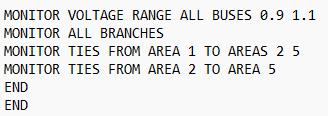
\includegraphics[scale=0.65]{mon.png}
   \caption{The monitored data file} 
   \label{fig:mon}
\end{figure}

\begin{figure}[H]
     \centering
   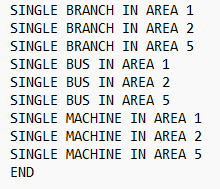
\includegraphics[scale=0.65]{con.png}
   \caption{The contingency data file} 
   \label{fig:con}
\end{figure}


For each of the studied scenarios, the API DFAX\_2 is used to construct different distribution factor data files corresponding to each .sav file, and the above defined .sub, .mon, .con configuration files. For each of the studied scenarios, by running the AC contingency calculation function ACCC\_WITH\_DSP\_3, the contingency solution output .acc files are obtained. 

Python code to conduct AC contingency calculation is:

\begin{python}
import psspy
psspy.case(r"""savnw.sav""")
psspy.fdns([0,1,0,0,0,0,99,0])
psspy.dfax_2([1,1,0],r"""savnw.sub""",r"""savnw.mon""",r"""savnw.con""",r"""savnw.dfx""")
psspy.accc_with_dsp_3(0.1,,[0,1,0,0,0,0,0,0,0,0,0],r"""CON""",r"""savnw.dfx""",r"""savnw.acc""","","","")
\end{python}

As can be seen from the code, the only option used to conduct the present AC Contingency Calculation for the studied topologies and scenarios is the area interchange adjustment flag (area interchange adjustment option setting) which is set to 1 to enable using tie line flows only in calculating area interchange. 

Using the contingency solution output file savnw.acc, the results is exported as an excel file for further analysis. The results exported are ACCC Analysis Summary, Monitored Branch Flow (MVA), Monitored Bus Voltage.

Python code to export AC contingency solution output file as excel is: 

\begin{python}
import psspy
import pssexcel
pssexcel.accc('savnw.acc', ['s','b','v'], colabel='',stype='contingency', busmsm=0.5, sysmsm=5.0,
                rating='a', namesplit=False,xlsfile='out.xlsx', sheet='', overwritesheet=True, show=False, ratecon='b',
                baseflowvio=False,basevoltvio=False, flowlimit=100.0, flowchange=0.0, voltchange=0.0,swdrating='a',
                swdratecon='b',baseswdflowvio=False,basenodevoltvio=False,overloadreport=False)
\end{python}

Detailed contingency analysis of all 7 topologies were carried out, and the results of the analysis were summarised as study reports for Topology 0 to Topology 6, and can be found \href{https://github.com/jessla89/PSSE-Contingency-Analysis}{here}. 

The contingency analysis was carried out for the 7 topologies for three types of faults and are single line open contingency fault, unit fault, and bus fault. The single line open contingency and unit faults are (N-1) contingency and takes out exactly one element of the system out of operation, whereas a single bus fault can take multiple elements of the interconnected system out of service. In the summary study for contingency analysis of the hypothetical SAVNW system, only (N-1) contingency cases are considered for reporting the loading and voltage violations. For each studied topology, the number of studied scenarios for which a branch gets overloaded due to a (N-1) contingency is summarised in Chapter ~\ref{chap:sum}. The Chapter ~\ref{chap:sum} also summarizes the number of studied scenarios for which a (N-1) contingency does not report a converged power flow solution.

\chapter{Topology Descriptions}
\label{chap:sum}

\section{Year 0 Topology 0}
Topology 0 of the system represents the system in the present year. For Year 0, Topology 0 only the reference load for an average hydrological scenario is tested for the contingency analysis and hence the number of scenarios tested is only one. The contingency analysis report for the hypothetical SAVNW system for Year 0 Topology 0 reporting the (N-1) contingencies along with the bus faults can be found \href{https://github.com/jessla89/PSSE-Contingency-Analysis}{here}. For the converged (N-1) contingencies the branches and buses violating the threshold are reported. The system single line diagram in the present year (at the beginning of the planning horizon) is as shown in Figure ~\ref{fig:y0t0}.

\begin{figure}[H]
\centering
\includegraphics[scale=0.57]{y0t0}
\caption{System Single Line Diagram in Year 0, Topology 0} 
\label{fig:y0t0}
\end{figure}


\section{Year 1 Topology 1}
Topology 1 is the system in Year 1 with solar farm in service with the addition of transformer to connect to the main system. For Year 1 Topology 1, there are 9 scenarios studied to account for the intermittent behaviour of the solar farm with 3 outputs along with the three load forecasts: low load forecast (LLS); reference load forecast (RLS); and high load forecast (HLS).
The contingency analysis report for the hypothetical SAVNW system for Year 1 Topology 1 reporting the (N-1) contingencies along with the bus faults can be found \href{https://github.com/jessla89/PSSE-Contingency-Analysis/blob/main/pssecontingency_topology_1.pdf}{here}. The system single line diagram in Year 1 with the addition of solar farm highlighted is as shown in Figure ~\ref{fig:y1t1}.

\begin{figure}[H]
\centering
\includegraphics[scale=0.57]{y1t1}
\caption{System Single Line Diagram in Year 1, Topology 1} 
\label{fig:y1t1}
\end{figure}

\section{Year 2 Topology 2}
Topology 2 is the system in Year 2  with the same system as Year 1 with increased load in all areas and hence single line diagram for Topology 2 is the same as that for Topology 1. Similar to Year 1 Topology 1, there are 9 scenarios studied for Year 2 Topology 2. 
The contingency analysis report for the hypothetical SAVNW system for Year 2 Topology 2 reporting the (N-1) contingencies along with the bus faults can be found \href{https://github.com/jessla89/PSSE-Contingency-Analysis/blob/main/pssecontingency_topology_2.pdf}{here}. 

\section{Year 3 Topology 3}
Topology 3 is the system in Year 3 with a new Hydro generator coming online at Bus 212 with transformer to connect to the system at Bus 201 without transmission system upgrades. For year 3, Topology 3, 27 scenarios are studied by accounting intermittency of solar and hydrological conditions with 3 generator outputs each along with 3 load forecasts. 
The contingency analysis report for the hypothetical SAVNW system for Year 3 Topology 3 reporting the (N-1) contingencies along with the bus faults can be found \href{https://github.com/jessla89/PSSE-Contingency-Analysis/blob/main/pssecontingency_topology_3.pdf}{here}. The system single line diagram in Year 3 with the addition of hydro generator highlighted is as shown in Figure ~\ref{fig:y3t3}.


\begin{figure}[H]
\centering
\includegraphics[scale=0.69]{y3t3}
\caption{System Single Line Diagram in Year 3, Topology 3} 
\label{fig:y3t3}
\end{figure}

\section{Year 3 Topology 4}
Topology 4 is the system in Year 3 with the Hydro generator coming online at Bus 212 with the completion of multiple transmission system upgrades. From the last Long Term Plan the transmission upgrades that are expected to be completed are the addition of transmission lines 3001-3003(2), 3005-3007(2), and 153-154(3), and Transformers 202-203(2), 204-205(2). Similar to Year 3 Topology 3, there are 27 scenarios studied for Year 3, Topology 4. 
The contingency analysis report for the hypothetical SAVNW system for Year 3 Topology 4 reporting the (N-1) contingencies along with the bus faults can be found \href{https://github.com/jessla89/PSSE-Contingency-Analysis/blob/main/pssecontingency_topology_4.pdf}{here}. The system single line diagram in Year 3 with the addition of hydro generator with transmission upgrade highlighted is as shown in Figure ~\ref{fig:y3t4}. 

\begin{figure}[H]
\centering
\includegraphics[scale=0.53]{y3t4}
\caption{System Single Line Diagram in Year 3, Topology 4} 
\label{fig:y3t4}
\end{figure}

\section{Year 4 Topology 5}
Topology 5 is the system in Year 4 with the wind farm in area 5 coming online with the grid transformer to connect to the main grid. There are 81 scenarios studied for this scenario for Year 4, Topology 5 by accounting for intermittency of solar, wind and hydro generators along with 3 load forecasts. 
The contingency analysis report for the hypothetical SAVNW system for Year 4 Topology 5 reporting the (N-1) contingencies along with the bus faults can be found \href{https://github.com/jessla89/PSSE-Contingency-Analysis/blob/main/pssecontingency_topology_5.pdf}{here}. The system single line diagram in Year 4 with the addition of Wind generator highlighted is as shown in Figure ~\ref{fig:y4t5}.

\begin{figure}[h!]
\centering
\includegraphics[scale=0.57]{year4top5}
\caption{System Single Line Diagram in Year 4, Topology 5} 
\label{fig:y4t5}
\end{figure}

\section{Year 5 Topology 6}

Topology 6 is the system in Year 5 without any new resource addition or transmission upgrades with increased load in all areas, hence, the single line diagram for Year 5 is same as the one for Year 4. Similar to Year 4, Topology 5, there are 81 scenarios studied for Year 5, Topology 6. 
The contingency analysis report for the hypothetical SAVNW system for Year 5 Topology 6 reporting the (N-1) contingencies along with the bus faults can be found \href{https://github.com/jessla89/PSSE-Contingency-Analysis/blob/main/pssecontingency_topology_6.pdf}{here}.


\chapter{Topology Summary - Non Convergences}
\label{chap:nonconv}

\section{Year 0 Topology 0}

The (N-1) contingencies for which the load flow did not converge for Year 0 Topology 0 are the unit fault contingency UNIT 206(1) and single open line contingency SING OPN LIN 14 205-206(1).

\section{Year 1 Topology 1}

For Year 1 Topology 1, the (N-1) contingencies for which the load flow did not converge are tabulated in Table \ref{count_blown_y1t1} with the corresponding count of scenarios. It can be seen from Table \ref{count_blown_y1t1} that the load flow did not converge for the contingencies UNIT 206(1) and SING OPN LIN   15 205-206(1) for 7 out of the 9 studied scenarios. 

\begin{table}[H]

\caption{Count of scenarios for which (N-1) contingencies failed to converge -  Year 1, Topology 1}
\label{count_blown_y1t1}
\centering
\scalebox{0.8}{\begin{tabular}{lr}
\toprule
Contingency & Count of Scenarios \\
\midrule
UNIT 206(1) & 7 \\
SING OPN LIN   15 205-206(1) & 7 \\
\bottomrule
\end{tabular}}

\end{table}

\section{Year 2 Topology 2}

For Year 2 Topology 2, the (N-1) contingencies for which the load flow did not converge are tabulated in Table \ref{y2t2cb} with the corresponding count of scenarios. It can be seen from Table \ref{y2t2cb} that the load flow did not converge for the contingencies UNIT 206(1) and SING OPN LIN   15 205-206(1) for any of the 9 studies scenarios, followed by SING OPN LIN   10 201-205(\&1) for  4, SING OPN LIN   12 202-203(1) for 1 of the 9 studied scenarios. 

\begin{table}[H]
\caption{Count of scenarios for which (N-1) contingencies failed to converge - Year 2, Topology 2}
\label{y2t2cb}


\centering
\scalebox{0.8}{\begin{tabular}{lr}
\toprule
Contingency & Count of Scenarios \\
\midrule
SING OPN LIN   15 205-206(1) & 9 \\
UNIT 206(1) & 9 \\
SING OPN LIN   10 201-205(\&1) & 4 \\
SING OPN LIN   12 202-203(1) & 1 \\
\bottomrule
\end{tabular}}
\end{table}

\section{Year 3 Topology 3}

For Year 3 Topology 3, the (N-1) contingencies for which the load flow did not converge are tabulated in Table \ref{y3t3cb} with the corresponding count of scenarios. It can be seen from Table \ref{y3t3cb} that the load flow did not converge for the contingencies UNIT 206(1), SING OPN LIN   16 205-206(1), SING OPN LIN   10 201-205(\&1) for any of the 27 studied scenarios. Rest of the contingencies and the number of scenarios for which the load flow did not converge for Year 3, Topology 3 is as shown in Table \ref{y3t3cb}.  

\begin{table}[H]
\caption{Count of scenarios for which (N-1) contingencies failed to converge - Year 3, Topology 3}
\label{y3t3cb}
\centering
\scalebox{0.8}{\begin{tabular}{lr}
\toprule
Contingency & Count of Scenarios \\
\midrule
UNIT 206(1) & 27 \\
SING OPN LIN   16 205-206(1) & 27 \\
SING OPN LIN   10 201-205(\&1) & 27 \\
SING OPN LIN   13 202-203(1) & 20 \\
SING OPN LIN   9 201-202(1) & 17 \\
SING OPN LIN   6 152-153(1) & 10 \\
SING OPN LIN   4 151-152(1) & 4 \\
SING OPN LIN   5 151-152(2) & 4 \\
SING OPN LIN   18 3001-3003(1) & 1 \\
\bottomrule
\end{tabular}}
\end{table}


\section{Year 3 Topology 4}

For Year 3 Topology 4, the (N-1) contingencies for which the load flow did not converge are tabulated in Table \ref{y3t4cb} with the corresponding count of scenarios. It can be seen from Table \ref{y3t4cb} that the load flow did not converge for the contingency SING OPN LIN   11 201-204(1) for 18 out of the 27 studied scenarios, followed by the contingencies SING OPN LIN   20 205-206(1) and UNIT 206(1) reporting nonconvergence 17 times each. The contingency SING OPN LIN   10 201-202(1) reported a nonconvergence for 1 studied scenario.  

\begin{table}[H]
\caption{Count of scenarios for which (N-1) contingencies failed to converge - Year 3, Topology 4}
\label{y3t4cb}
\centering
\scalebox{0.8}{\begin{tabular}{lr}
\toprule
Contingency & Count of Scenarios \\
\midrule
SING OPN LIN   11 201-204(1) & 18 \\
SING OPN LIN   20 205-206(1) & 17 \\
UNIT 206(1) & 17 \\
SING OPN LIN   10 201-202(1) & 1 \\
\bottomrule
\end{tabular}}
\end{table}

\section{Year 4 Topology 5}

For Year 4 Topology 5, the (N-1) contingencies for which the load flow did not converge are tabulated in Table \ref{y4t5cb} with the corresponding count of scenarios. It can be seen from Table \ref{y4t5cb} that the load flow did not converge for the contingency SING OPN LIN   11 201-204(1) for 72 out of the 81 studied scenarios, followed by the contingencies SING OPN LIN   20 205-206(1) and UNIT 206(1) reporting nonconvergence 71 times each. Rest of the contingencies and the number of scenarios for which the load flow did not converge for Year 4, Topology 5 is as shown in Table \ref{y4t5cb}.  

\begin{table}[H]
\caption{Count of scenarios for which (N-1) contingencies failed to converge - Year 4, Topology 5}
\label{y4t5cb}
\centering
\scalebox{0.8}{\begin{tabular}{lr}
\toprule
Contingency & Count of Scenarios \\
\midrule
SING OPN LIN   11 201-204(1) & 72 \\
SING OPN LIN   20 205-206(1) & 71 \\
UNIT 206(1) & 71 \\
SING OPN LIN   10 201-202(1) & 25 \\
SING OPN LIN   6 152-153(1) & 7 \\
SING OPN LIN   5 151-152(2) & 6 \\
SING OPN LIN   4 151-152(1) & 6 \\
\bottomrule
\end{tabular}}
\end{table}


\section{Year 5 Topology 6}

For Year 5 Topology 6, the (N-1) contingencies for which the load flow did not converge are tabulated in Table \ref{y5t6cb} with the corresponding count of scenarios. It can be seen from Table \ref{y5t6cb} that the load flow did not converge for the contingencies SING OPN LIN   20 205-206(1), SING OPN LIN   11 201-204(1), UNIT 206(1) for any of the 81 studied scenarios. Rest of the contingencies and the number of scenarios for which the load flow did not converge for Year 5, Topology 6 is as shown in Table \ref{y5t6cb}.  

\begin{table}[H]
\caption{Count of scenarios for which (N-1) contingencies failed to converge - Year 5, Topology 6}
\label{y5t6cb}
\centering
\scalebox{0.8}{\begin{tabular}{lr}
\toprule
Contingency & Count of Scenarios \\
\midrule
SING OPN LIN   20 205-206(1) & 81 \\
SING OPN LIN   11 201-204(1) & 81 \\
UNIT 206(1) & 81 \\
SING OPN LIN   10 201-202(1) & 54 \\
SING OPN LIN   6 152-153(1) & 31 \\
SING OPN LIN   5 151-152(2) & 30 \\
SING OPN LIN   4 151-152(1) & 30 \\
\bottomrule
\end{tabular}}
\end{table} 

\section{Result Summary}

Following are the observations obtained by studying the Topologies for non convergence 

\begin{itemize}
\item The contingencies UNIT 206(1) and SING OPN LIN 205-206(1) reported the most number of non convergence. This is because the contingencies UNIT 206(1) and SING OPN LIN 205-206(1) takes the generator connected to Bus 206 out of operation. As the largest load in the network is connected to the Bus 205, it is evident that the removal of this generator to serve the loads will results in a large unbalance resulting in nonconvergence of the load flow. 
In order to ensure the system is able to withstand this unbalance, feasibility studies needed to be conducted on the system for a possible addition of a new Generator Transformer unit to serve the load in this Area closer to the load center. 
\item The contingency SING OPN LIN 201-202(1) nonconvergence can be understood by looking at the single line diagram. The line 201-202(1) is one of the line for the generator connected at Buses 211 and 212 to serve the loads in Area 2. When this line is lost due to a contingency, the capability of the generators connected at Bus 211 and 212 to serve the load of Area reduces, leading to load flow nonconvergence. 
\item Similar to the line outage 201-202(1) reducing the systems capability to transfer power from generators connected at Bus 211 and 212 to serve the loads connected at Bus 203 and 205, the single line contingency 202-203(1) also causes the systems capability to transfer power from Generators at Buses 211 to 212 and hence the generator unable to transfer the power and causing the load flow not to converge. 
\item The line SING OPN LIN 201-205(\&1) is multisegmented single line contingency which had reported nonconvergence in Year 2 and Year 3. In Year 3, as part of the transmission upgrade, the second part of the segment would be upgraded with an additional transformer in parallel to the existing transformer to increase the capacity of transfer. When the upgrade would be complete in Year 3, the planning study shows that the outage of the single line branch 201-204(1) only reports nonconvergence, calling for upgrade of the line to have back up path for transfer of power from generating units connected at Bus 211 and 212. 
\item The single line contingencies in Area 1 whose outages could cause the nonconvergence of load flow obtained from the contingency analysis are corresponding outages of branches 151-152(1), 151-152(2), and 152-153(1). The amount of power that transferred through these branches are very high. These branches would become a path of power transfer from Area 2 generation to Area 1 back to Area 2 loads. These branch outages only report nonconvergence after the 3rd year when the hydro generator at Bus 212 becomes operational. The lack of transmission upgrade in Area 2 due to various reasons for the addition of generating unit at Bus 212 would be the cause of these nonconvergence in area 1 in branches 151-152(1), 151-152(2), and 152-153(1). 
\item There would only be 1 time when the contingency SING OPN LIN 3001-3003(1) would report a nonconvergence would be before the transmission upgrade of parallel line 3001-3003(2) would have been added to the system.

\end{itemize} 


\chapter{Topology Summary - Loading Violations}
\label{chap:ovrld}

\section{Introduction}

In this Chapter, for each of the topologies, the number of times a branch reports a loading greater than 100\% of its rating 2 is tabulated along with the contingecies causing the reported loading violation.

\section{Year 0 Topology 0}

For Year 0 Topology 0, the branch reporting the most number of overload violations is the branch 3001-3003(1), reporting violations for (N-1) contingencies SING OPN LIN   1 101-151(1) and UNIT 101(1), followed by the branch 153-154(1) reporting a violation for (N-1) contingency SING OPN LIN   12 202-203(1) as given in Table \ref{y0t0ol}.


\begin{table}[H]
\caption{Branch overload violation count with contingencies - Year 0, Topology 0}
\label{y0t0ol}

\centering
\scalebox{0.8}{\begin{tabular}{llrrrr}
\toprule
Branch & Contingency & Count \\
\midrule
3001-3003(1) & SING OPN LIN   1 101-151(1), UNIT 101(1) & 2 \\
153-154(1) & SING OPN LIN   11 202-203(1) & 1 \\
\bottomrule
\end{tabular}}
\end{table}


\section{Year 1 Topology 1}

For Year 1 Topology 1, the branch reporting the most number of overload violations is the branch 3001-3003(1), reporting violations for (N-1) contingencies SING OPN LIN   1 101-151(1), UNIT 101(1), SING OPN LIN   15 205-206(1), and UNIT 206(1), followed by the branch 153-154(1) reporting violations for (N-1) contingencies SING OPN LIN   12 202-203(1), SING OPN LIN   10 201-205(\&1), SING OPN LIN   15 205-206(1), UNIT 206(1) as given in Table \ref{y1t1ol}. Rest of the branches and the corresponding contingencies for which violations are reported can be referred from Table \ref{y1t1ol}. 

\begin{table}[H]
\caption{Branch overload violation count with contingencies - Year 1, Topology 1}
\label{y1t1ol}
\centering
\scalebox{0.8}{\begin{tabular}{llr}
\toprule
Branch & Contingencies & Overload Count \\
\midrule
3001-3003(1) & SING OPN LIN   1 101-151(1), UNIT 101(1), SING OPN LIN   15 205-206(1), UNIT 206(1) & 22 \\
153-154(1) & SING OPN LIN   12 202-203(1), SING OPN LIN   10 201-205(\&1), SING OPN LIN   15 205-206(1), UNIT 206(1) & 14 \\
205-206(1) & SING OPN LIN   11 201-211(1), UNIT 211(1) & 8 \\
154-205(1) & SING OPN LIN   6 152-153(1) & 5 \\
3005-3007(1) & SING OPN LIN   15 205-206(1), UNIT 206(1) & 4 \\
101-151(1) & SING OPN LIN   2 102-151(1), UNIT 102(1) & 2 \\
\bottomrule
\end{tabular}}
\end{table}

\section{Year 2 Topology 2}

For Year 2 Topology 2, the branch reporting the most number of overload violations is the branch 3001-3003(1), reporting violations for (N-1) contingencies SING OPN LIN   1 101-151(1) and UNIT 101(1), followed by the branch 205-206(1) reporting violations for (N-1) contingencies SING OPN LIN   11 201-211(1), UNIT 211(1) as given in Table \ref{y2t2ol}. Rest of the branches and the corresponding contingencies for which violations are reported can be referred from Table \ref{y2t2ol}. 

\begin{table}[H]
\caption{Branch overload violation count with contingencies - Year 2, Topology 2}
\label{y2t2ol}
\centering
\scalebox{0.8}{\begin{tabular}{llr}
\toprule
Branch & Contingencies & Overload Count \\
\midrule
3001-3003(1) & SING OPN LIN   1 101-151(1), UNIT 101(1) & 18 \\
205-206(1) & SING OPN LIN   11 201-211(1), UNIT 211(1) & 16 \\
153-154(1) & SING OPN LIN   10 201-205(\&1), SING OPN LIN   12 202-203(1) & 10 \\
154-205(1) & SING OPN LIN   6 152-153(1) & 8 \\
101-151(1) & SING OPN LIN   2 102-151(1), UNIT 102(1) & 6 \\
153-154(2) & SING OPN LIN   12 202-203(1) & 3 \\
154-203(1) & SING OPN LIN   6 152-153(1) & 2 \\
\bottomrule
\end{tabular}}
\end{table} 

\section{Year 3 Topology 3}

For Year 3 Topology 3, the branch reporting the most number of overload violations is the branch 3001-3003(1), reporting violations for (N-1) contingencies SING OPN LIN   1 101-151(1), UNIT 101(1), SING OPN LIN   6 152-153(1), SING OPN LIN   23 3004-3005(1), SING OPN LIN   27 3008-3018(1), UNIT 3018(1), SING OPN LIN   17 3001-3002(1), and SING OPN LIN   20 3002-3004(1) as given in Table \ref{y3t3ol}. Rest of the branches and the corresponding contingencies for which violations are reported can be referred from Table \ref{y3t3ol}. 

\begin{table}[H]
\caption{Branch overload violation count with contingencies - Year 3, Topology 3}
\label{y3t3ol}
\centering
\scalebox{0.8}{\begin{tabular}{lp{18cm}r}
\toprule
Branch & Contingencies & Overload Count \\
\midrule
3001-3003(1) & SING OPN LIN   1 101-151(1), UNIT 101(1), SING OPN LIN   6 152-153(1), SING OPN LIN   23 3004-3005(1), SING OPN LIN   27 3008-3018(1), UNIT 3018(1), SING OPN LIN   17 3001-3002(1), SING OPN LIN   20 3002-3004(1), BASE CASE & 93 \\
3005-3007(1) & SING OPN LIN   13 202-203(1), SING OPN LIN   26 3005-3008(1), SING OPN LIN   1 101-151(1), UNIT 101(1), BASE CASE, SING OPN LIN   7 153-154(1) & 46 \\
101-151(1) & SING OPN LIN   2 102-151(1), UNIT 102(1) & 44 \\
153-154(1) & SING OPN LIN   13 202-203(1), SING OPN LIN   8 153-154(2), BASE CASE & 30 \\
153-154(2) & SING OPN LIN   13 202-203(1), SING OPN LIN   7 153-154(1), BASE CASE & 22 \\
154-203(1) & SING OPN LIN   6 152-153(1), SING OPN LIN   7 153-154(1) & 18 \\
3003-3005(1) & SING OPN LIN   1 101-151(1), UNIT 101(1) & 18 \\
3003-3005(2) & SING OPN LIN   1 101-151(1), UNIT 101(1) & 18 \\
202-203(1) & SING OPN LIN   6 152-153(1), BASE CASE & 13 \\
154-205(1) & SING OPN LIN   6 152-153(1) & 11 \\
204-205(1) & BASE CASE, SING OPN LIN   9 201-202(1) & 7 \\
203-205(1) & SING OPN LIN   6 152-153(1) & 3 \\
203-205(2) & SING OPN LIN   6 152-153(1) & 3 \\
\bottomrule
\end{tabular}}
\end{table}

It can be seen that for Year 3, Topology 3, a branch loading greater than 100\% was reported for the base case as well. 

\section{Year 3 Topology 4}

For Year 3 Topology 4, the branches reporting the most number of overload violations are the branches 3001-3003(1) and 3001-3003(2), reporting violations for (N-1) contingencies SING OPN LIN   1 101-151(1), UNIT 101(1), SING OPN LIN   20 205-206(1) and UNIT 206(1) as given in Table \ref{y3t4ol}. Rest of the branches and the corresponding contingencies for which violations are reported can be referred from Table \ref{y3t4ol}. 

\begin{table}[H]
\caption{Branch overload violation count with contingencies - Year 3, Topology 4}
\label{y3t4ol}
\centering
\scalebox{0.8}{\begin{tabular}{llr}
\toprule
Branch & Contingencies & Overload Count \\
\midrule
3001-3003(1) & SING OPN LIN   1 101-151(1), UNIT 101(1), SING OPN LIN   20 205-206(1), UNIT 206(1) & 48 \\
3001-3003(2) & SING OPN LIN   1 101-151(1), UNIT 101(1), SING OPN LIN   20 205-206(1), UNIT 206(1) & 48 \\
101-151(1) & SING OPN LIN   2 102-151(1), UNIT 102(1) & 44 \\
154-203(1) & SING OPN LIN   6 152-153(1), SING OPN LIN   11 201-204(1) & 34 \\
3003-3005(1) & SING OPN LIN   1 101-151(1), UNIT 101(1), SING OPN LIN   20 205-206(1), UNIT 206(1) & 20 \\
3003-3005(2) & SING OPN LIN   1 101-151(1), UNIT 101(1), SING OPN LIN   20 205-206(1), UNIT 206(1) & 20 \\
154-205(1) & SING OPN LIN   6 152-153(1) & 19 \\
203-205(1) & SING OPN LIN   11 201-204(1), SING OPN LIN   6 152-153(1) & 16 \\
203-205(2) & SING OPN LIN   11 201-204(1), SING OPN LIN   6 152-153(1) & 16 \\
201-204(1) & SING OPN LIN   10 201-202(1) & 3 \\
\bottomrule
\end{tabular}}
\end{table}

\section{Year 4 Topology 5}

For Year 4 Topology 5, the branches reporting the most number of overload violations are the branches 3001-3003(1) and 3001-3003(2), reporting violations for (N-1) contingencies SING OPN LIN   1 101-151(1), UNIT 101(1), SING OPN LIN   20 205-206(1) and UNIT 206(1) as given in Table \ref{y4t5ol}. Rest of the branches and the corresponding contingencies for which violations are reported can be referred from Table \ref{y4t5ol}. 

\begin{table}[H]
\caption{Branch overload violation count with contingencies - Year 4, Topology 5}
\label{y4t5ol}
\centering
\scalebox{0.8}{\begin{tabular}{llr}
\toprule
Branch & Contingencies & Overload Count \\
\midrule
3001-3003(1) & SING OPN LIN   1 101-151(1), UNIT 101(1), SING OPN LIN   20 205-206(1), UNIT 206(1) & 164 \\
3001-3003(2) & SING OPN LIN   1 101-151(1), UNIT 101(1), SING OPN LIN   20 205-206(1), UNIT 206(1) & 164 \\
101-151(1) & SING OPN LIN   2 102-151(1), UNIT 102(1) & 162 \\
3003-3005(1) & SING OPN LIN   1 101-151(1), UNIT 101(1) & 90 \\
3003-3005(2) & SING OPN LIN   1 101-151(1), UNIT 101(1) & 90 \\
154-203(1) & SING OPN LIN   6 152-153(1), SING OPN LIN   11 201-204(1), BASE CASE & 89 \\
154-205(1) & SING OPN LIN   6 152-153(1), SING OPN LIN   10 201-202(1) & 68 \\
203-205(1) & SING OPN LIN   11 201-204(1), SING OPN LIN   6 152-153(1) & 42 \\
203-205(2) & SING OPN LIN   11 201-204(1), SING OPN LIN   6 152-153(1) & 42 \\
205-206(1) & SING OPN LIN   12 201-211(1), SING OPN LIN   13 201-212(1), UNIT 211(1), UNIT 212(1) & 36 \\
201-204(1) & SING OPN LIN   10 201-202(1) & 6 \\
\bottomrule
\end{tabular}}
\end{table}

\section{Year 5 Topology 6}

For Year 5 Topology 6, the branches reporting the most number of overload violations are the branches 3001-3003(1), 3001-3003(2) and 101-151(1) as given in Table \ref{y5t6ol}, with the branches 3001-3003(1) and 3001-3003(2) reporting violations for (N-1) contingencies SING OPN LIN   1 101-151(1) and UNIT 101(1), and the branch 101-151(1) reporting for (N-1) contingencies SING OPN LIN   2 102-151(1) and UNIT 102(1). Rest of the branches and the corresponding contingencies for which violations are reported can be referred from Table \ref{y5t6ol}. 

\begin{table}[H]
\caption{Branch overload violation count with contingencies - Year 5, Topology 6}
\label{y5t6ol}
\centering
\scalebox{0.8}{\begin{tabular}{llr}
\toprule
Branch & Contingencies & Overload Count \\
\midrule
3001-3003(1) & SING OPN LIN   1 101-151(1), UNIT 101(1) & 162 \\
3001-3003(2) & SING OPN LIN   1 101-151(1), UNIT 101(1) & 162 \\
101-151(1) & SING OPN LIN   2 102-151(1), UNIT 102(1) & 162 \\
3003-3005(1) & SING OPN LIN   1 101-151(1), UNIT 101(1) & 134 \\
3003-3005(2) & SING OPN LIN   1 101-151(1), UNIT 101(1) & 134 \\
205-206(1) & SING OPN LIN   12 201-211(1), SING OPN LIN   13 201-212(1), UNIT 211(1), UNIT 212(1) & 108 \\
154-203(1) & SING OPN LIN   6 152-153(1), BASE CASE & 68 \\
154-205(1) & SING OPN LIN   6 152-153(1) & 50 \\
203-205(1) & SING OPN LIN   6 152-153(1) & 30 \\
203-205(2) & SING OPN LIN   6 152-153(1) & 30 \\
201-204(1) & SING OPN LIN   10 201-202(1) & 3 \\
\bottomrule
\end{tabular}}
\end{table}

By the end of the Year 5, with the load increase in the system, it can be seen that a loading greater than 100\% was reported for base case as well. 

\section{Result Summary}

Observations regarding the overloading violations are
\begin{itemize}
\item The branch 3001-3003(1) is the branch reporting the most number of loading violations across all the studied topologies and scenarios. It was seen that except for year 3, topology 3 when the system is highly overloaded without any transmission transfer path back ups, the overloading of the branch 3001-3003(1) is caused due to an area swing generator outage, forcing dispatch of the system swing generator connected at Bus 3011 to balance the power flow. Here, the system swing generator is being dispatched than the reserves in the same area because of the AC contingency calculation parameter used for this study.
\item When either of the area swing generator goes out of service due to one of the following single line contingencies SING OPN LIN 1 101-151(1), UNIT 101(1), SING OPN LIN 20 205-206(1), UNIT 206(1), sensitivity analysis conducted shows that the generation from 3011 increases the loading on the branches 3001-3003(1) and when the transmission upgrade would be completed in Year 3, the overloading due to these contingencies extends to the parallel branch 3001-3003(2) as well. The transmission upgrade does not relieve the load on the branches as the capacity of the newly added branch is same as the already existing low-capacity branch, and the combined capacity of the two parallel branches are still not enough to bring the loading to less than 100\%. 
\item For the parallel branches 153-154(1) and 153-154(2), for Year 2, Topology 2, when the contingency single line open 202-203(1) was studied, the sensitivity analysis showed that the power flows through the branches 202 - 152(1), 152 - 153(1), 153 - 154(1), 153-154(2), and back to 154-203(1) and 154 to 205 to reach the main load center. The branches 153-154(1) and 153-154(2) being low capacity branches, reported a loading greater than 100\%.
\item For year 1, Topology 1 the loading violation is reported for the branch 205-206(1) for single line outage 201-211(1) and UNIT 211. Both of these contingencies essentially take the generating unit 211 out of service, resulting in the generating unit at 206 to generate more and hence resulting in overload in the transformer branch from 206 to 205. When the generator at Bus 212 comes into service in year 3, overloading of the branch 205-206(1) is also reported when single line contingencies that takes the generating unit at 212 out of service. 
\item When single line open occurs at the transformer branch 152-153(1) in various studied topologies, the path to transfer power from Bus 152 to 154 is open between 152 and 153. The sensitivity analysis indicates this results in increased flows to both ties to which the branch 152 is connected and from ties to which the branch 154 is connected. Among various studied topologies, the branches reporting a loading greater than 100\% for SING OPN LIN 152-153(1) are the branches 154-205(1), 154-203(1), 202-203(1), 204-205(1), 203-205(1) and 203-205(2). 
\item The overloading of Branch 3005-3007(1) in area 5 would be caused by SING OPN LIN 20 205-206(1) and UNIT 206(1), as the sensitivity analysis shows that, when these contingencies may occur, there would need to be additional generation needed from the system swing generator connected at Bus 3011, and hence causing the branch flows in the area 5 to increase.
\item For the studied topologies reporting loading greater than 100\% of the branch 101-151(1) would be caused by the contingency that would take the generator at Bus 102 out of service. This is because the area swing generator bus connected at Bus 101 would compensate for the loss generation at Bus 102.
\end{itemize}


\chapter{Topology Summary - Upper Emergency Voltage Violations}
\label{chap:upemvol}

\section{Year 0 Topology 0}

For (N-1) contingency cases, for Year 0, Topology 0, there were no buses reporting an upper emergency voltage violation of bus voltage greater than 1.1 PU. 

\section{Year 1 Topology 1}
For Year 1, Topology 1, the AC contingency calculation showed the Bus at 211 violating the upper emergency voltage limit of 1.1 PU as can be seen in Table ~\ref{y1t1hv}. The two cases in which the bus 211 reported a voltage greater than the upper emergency rating are for faults that takes the generator at Bus 206 out of service corresponding to the contingencies SING OPN LIN   15 205-206(1) and UNIT 206(1). 


\begin{table}[H]
\caption{Upper emergency voltage range violation counts - Buses with Contingencies - Year 1, Topology 1}
\label{y1t1hv}
\centering
\scalebox{0.8}{\begin{tabular}{llr}
\toprule
Bus & Contingencies & Upper violation counts \\
\midrule
211 & SING OPN LIN   15 205-206(1), UNIT 206(1) & 8 \\
\bottomrule
\end{tabular}}
\end{table}


\section{Year 2 Topology 2}

No upper voltage violations were reported for Year 2, Topology 2.

\section{Year 3 Topology 3}

For Year 3, Topology 3, the AC contingency calculation showed the Buses 211 and 212 violating the upper emergency voltage limit of 1.1 PU as can be seen in Table ~\ref{y3t3hv}.

\begin{table}[H]
\caption{Upper emergency voltage range violation counts - Buses with Contingencies - Year 3, Topology 3}
\label{y3t3hv}
\centering
\scalebox{0.8}{\begin{tabular}{lp{18cm}r}
\toprule
Bus & Contingencies & Upper violation counts \\
\midrule
211 & SING OPN LIN   6 152-153(1), SING OPN LIN   4 151-152(1), SING OPN LIN   5 151-152(2), SING OPN LIN   7 153-154(1), SING OPN LIN   18 3001-3003(1) & 14 \\
212 & SING OPN LIN   6 152-153(1), SING OPN LIN   4 151-152(1), SING OPN LIN   5 151-152(2), SING OPN LIN   7 153-154(1), SING OPN LIN   18 3001-3003(1) & 14\\
\bottomrule
\end{tabular}}
\end{table}

\section{Year 3 Topology 4}

For Year 3, Topology 4, the AC contingency calculation showed the Buses 211 and 212 violating the upper emergency voltage limit of 1.1 PU as can be seen in Table ~\ref{y3t4hv}. 

\begin{table}[H]
\caption{Upper emergency voltage range violation counts - Buses with Contingencies - Year 3, Topology 4}
\label{y3t4hv}
\centering
\scalebox{0.8}{\begin{tabular}{llr}
\toprule
Bus & Contingencies & Upper violation counts \\
\midrule
211 & SING OPN LIN   20 205-206(1), UNIT 206(1), SING OPN LIN   10 201-202(1) & 6 \\
212 & SING OPN LIN   20 205-206(1), UNIT 206(1), SING OPN LIN   10 201-202(1) & 6 \\
\bottomrule
\end{tabular}}
\end{table}

\section{Year 4 Topology 5}

For Year 4, Topology 5, the AC contingency calculation showed the Buses 211 and 212 violating the upper emergency voltage limit of 1.1 PU as can be seen in Table ~\ref{y4t5hv}. 

\begin{table}[H]
\caption{Upper emergency voltage range violation counts - Buses with Contingencies - Year 4, Topology 5}
\label{y4t5hv}
\centering
\scalebox{0.8}{\begin{tabular}{lp{18cm}r}
\toprule
Bus & Contingencies & Upper violation counts \\
\midrule
211 & SING OPN LIN   10 201-202(1), SING OPN LIN   4 151-152(1), SING OPN LIN   5 151-152(2), SING OPN LIN   6 152-153(1), SING OPN LIN   20 205-206(1), UNIT 206(1) & 49\\
212 & SING OPN LIN   10 201-202(1), SING OPN LIN   4 151-152(1), SING OPN LIN   5 151-152(2), SING OPN LIN   6 152-153(1), SING OPN LIN   20 205-206(1), UNIT 206(1) & 49\\
\bottomrule
\end{tabular}}
\end{table}

\section{Year 5 Topology 6}

For Year 5, Topology 6, the AC contingency calculation showed the Buses 211 and 212 violating the upper emergency voltage limit of 1.1 PU as can be seen in Table ~\ref{y5t6hv}. 

\begin{table}[H]
\caption{Upper emergency voltage range violation counts - Buses with Contingencies - Year 5, Topology 6}
\label{y5t6hv}
\centering
\scalebox{0.8}{\begin{tabular}{lp{18cm}r}
\toprule
Bus & Contingencies & Upper violation counts \\

\midrule
211 & SING OPN LIN   4 151-152(1), SING OPN LIN   5 151-152(2), SING OPN LIN   6 152-153(1), SING OPN LIN   2 102-151(1), SING OPN LIN   7 153-154(1), SING OPN LIN   8 153-154(2), SING OPN LIN   9 153-154(3), SING OPN LIN   14 202-203(1), SING OPN LIN   15 202-203(2), SING OPN LIN   18 204-205(1), SING OPN LIN   19 204-205(2), SING OPN LIN   26 3003-3005(1), SING OPN LIN   27 3003-3005(2), SING OPN LIN   35 3008-3018(1), UNIT 102(1), UNIT 3018(1), SING OPN LIN   10 201-202(1) & 82 \\
212 & SING OPN LIN   4 151-152(1), SING OPN LIN   5 151-152(2), SING OPN LIN   6 152-153(1), SING OPN LIN   2 102-151(1), SING OPN LIN   7 153-154(1), SING OPN LIN   8 153-154(2), SING OPN LIN   9 153-154(3), SING OPN LIN   14 202-203(1), SING OPN LIN   15 202-203(2), SING OPN LIN   18 204-205(1), SING OPN LIN   19 204-205(2), SING OPN LIN   26 3003-3005(1), SING OPN LIN   27 3003-3005(2), SING OPN LIN   35 3008-3018(1), UNIT 102(1), UNIT 3018(1), SING OPN LIN   10 201-202(1) & 82 \\

\bottomrule
\end{tabular}}
\end{table}

\section{Result Summary}

In all the topologies studied, the upper emergency voltage violations are reported by the generator buses 211 and 212 is due to these buses regulating the voltage of the bus 201. In the study the buses 211 and 212 are set to regulate the voltage at the bus 201 to 1.04 PU. It was seen that across all the studied topologies and scenarios the bus 201 never violates the upper or lower emergency or normal voltage ratings. 


\chapter{Topology Summary - Lower Emergency Voltage Violations}
\label{chap:lowemvol}
\section{Year 0 Topology 0}

For Year 0, Topology 0, there were no buses reporting lower emergency voltage violation for a tested (N-1) contingency. 

\section{Year 1 Topology 1}

For Year 1, Topology 1, the AC contingency calculation showed the Buses 103, 154, 203, 205, 206 and 3008 violating the lower emergency voltage limit of 0.9 PU as can be seen in Table ~\ref{y1t1lv}.

\begin{table}[H]
\caption{Lower emergency voltage violation counts - Buses with Contingencies - Year 1, Topology 1}
\label{y1t1lv}
\centering
\scalebox{0.8}{\begin{tabular}{llr}
\toprule
Bus & Contingencies & Lower violation counts \\
\midrule
103 & SING OPN LIN   10 201-205(\&1), SING OPN LIN   15 205-206(1), UNIT 206(1) & 14 \\
154 & SING OPN LIN   10 201-205(\&1), SING OPN LIN   15 205-206(1), UNIT 206(1) & 14 \\
205 & SING OPN LIN   10 201-205(\&1), SING OPN LIN   15 205-206(1), UNIT 206(1) & 14 \\
3008 & SING OPN LIN   10 201-205(\&1), SING OPN LIN   15 205-206(1), UNIT 206(1) & 10 \\
206 & UNIT 206(1) & 4 \\
203 & SING OPN LIN   10 201-205(\&1) & 2 \\
\bottomrule
\end{tabular}}
\end{table}

\section{Year 2 Topology 2}

For Year 2, Topology 2, the AC contingency calculation showed the Buses 103, 153,154, 203, 204, 205, 3007 and 3008 violating the lower emergency voltage limit of 0.9 PU as can be seen in Table ~\ref{y2t2lv}.

\begin{table}[H]
\caption{Lower emergency voltage violation counts - Buses with Contingencies - Year 2, Topology 2}
\label{y2t2lv}
\centering
\scalebox{0.8}{\begin{tabular}{lp{18cm}r}
\toprule
Bus & Contingencies & Lower violation counts \\
\midrule
103 & SING OPN LIN   12 202-203(1), SING OPN LIN   6 152-153(1), SING OPN LIN   9 201-202(1), SING OPN LIN   10 201-205(\&1) & 20 \\
154 & SING OPN LIN   12 202-203(1), SING OPN LIN   6 152-153(1), SING OPN LIN   9 201-202(1), SING OPN LIN   10 201-205(\&1) & 20 \\
203 & SING OPN LIN   12 202-203(1), SING OPN LIN   10 201-205(\&1) & 14 \\
205 & SING OPN LIN   6 152-153(1), SING OPN LIN   12 202-203(1), SING OPN LIN   10 201-205(\&1) & 12 \\
3008 & SING OPN LIN   12 202-203(1), SING OPN LIN   10 201-205(\&1) & 8 \\
153 & SING OPN LIN   6 152-153(1) & 4 \\
204 & SING OPN LIN   12 202-203(1) & 2 \\
3007 & SING OPN LIN   10 201-205(\&1) & 2 \\
\bottomrule
\end{tabular}}
\end{table}

\section{Year 3 Topology 3}

For Year 3, Topology 3, the AC contingency calculation showed the Buses 103, 153,154, 202, 203, 204, 205, 206, 3005, 3006, 3007, 3008 and 3018 violating the lower emergency voltage limit of 0.9 PU as can be seen in Table ~\ref{y3t3lv}.

\begin{table}[H]
\caption{Lower emergency voltage violation counts - Buses with Contingencies - Year 3, Topology 3}
\label{y3t3lv}
\centering
\scalebox{0.8}{\begin{tabular}{lp{18cm}r}
\toprule
Bus & Contingencies & Lower violation counts \\
\midrule

154 & SING OPN LIN   13 202-203(1), SING OPN LIN   6 152-153(1), SING OPN LIN   9 201-202(1), SING OPN LIN   7 153-154(1), SING OPN LIN   8 153-154(2), SING OPN LIN   18 3001-3003(1), SING OPN LIN   4 151-152(1), SING OPN LIN   5 151-152(2), SING OPN LIN   26 3005-3008(1), SING OPN LIN   27 3008-3018(1), UNIT 3018(1), SING OPN LIN   1 101-151(1), SING OPN LIN   2 102-151(1), SING OPN LIN   3 103-154(1), SING OPN LIN   14 203-205(1), SING OPN LIN   15 203-205(2), SING OPN LIN   17 3001-3002(1), SING OPN LIN   20 3002-3004(1), SING OPN LIN   21 3003-3005(1), SING OPN LIN   22 3003-3005(2), SING OPN LIN   23 3004-3005(1), SING OPN LIN   24 3005-3006(1), UNIT 101(1), UNIT 102(1), UNIT 103(1) & 188 \\

205 & SING OPN LIN   13 202-203(1), SING OPN LIN   9 201-202(1), SING OPN LIN   6 152-153(1), SING OPN LIN   7 153-154(1), SING OPN LIN   4 151-152(1), SING OPN LIN   5 151-152(2), SING OPN LIN   8 153-154(2), SING OPN LIN   18 3001-3003(1), SING OPN LIN   1 101-151(1), SING OPN LIN   2 102-151(1), SING OPN LIN   3 103-154(1), SING OPN LIN   14 203-205(1), SING OPN LIN   15 203-205(2), SING OPN LIN   17 3001-3002(1), SING OPN LIN   20 3002-3004(1), SING OPN LIN   21 3003-3005(1), SING OPN LIN   22 3003-3005(2), SING OPN LIN   23 3004-3005(1), SING OPN LIN   26 3005-3008(1), SING OPN LIN   27 3008-3018(1), UNIT 101(1), UNIT 102(1), UNIT 3018(1), UNIT 103(1) & 150 \\

3008 & SING OPN LIN   13 202-203(1), SING OPN LIN   6 152-153(1), SING OPN LIN   9 201-202(1), SING OPN LIN   4 151-152(1), SING OPN LIN   5 151-152(2), SING OPN LIN   18 3001-3003(1), SING OPN LIN   1 101-151(1), SING OPN LIN   7 153-154(1), SING OPN LIN   8 153-154(2), SING OPN LIN   23 3004-3005(1), SING OPN LIN   26 3005-3008(1), SING OPN LIN   27 3008-3018(1), UNIT 101(1), UNIT 3018(1) & 80 \\

103 & SING OPN LIN   13 202-203(1), SING OPN LIN   6 152-153(1), SING OPN LIN   9 201-202(1), SING OPN LIN   4 151-152(1), SING OPN LIN   5 151-152(2), SING OPN LIN   7 153-154(1), SING OPN LIN   8 153-154(2), SING OPN LIN   27 3008-3018(1), UNIT 3018(1), SING OPN LIN   18 3001-3003(1), UNIT 103(1) & 68 \\

203 & SING OPN LIN   13 202-203(1), SING OPN LIN   9 201-202(1), SING OPN LIN   6 152-153(1), SING OPN LIN   4 151-152(1), SING OPN LIN   5 151-152(2), SING OPN LIN   7 153-154(1), SING OPN LIN   8 153-154(2), SING OPN LIN   18 3001-3003(1) & 50 \\

3007 & SING OPN LIN   13 202-203(1), SING OPN LIN   6 152-153(1), SING OPN LIN   9 201-202(1), SING OPN LIN   4 151-152(1), SING OPN LIN   5 151-152(2), SING OPN LIN   18 3001-3003(1), SING OPN LIN   1 101-151(1), SING OPN LIN   7 153-154(1), SING OPN LIN   27 3008-3018(1), UNIT 101(1), UNIT 3018(1) & 46 \\

153 & SING OPN LIN   6 152-153(1), SING OPN LIN   9 201-202(1) & 26 \\

3006 & SING OPN LIN   6 152-153(1) & 22 \\

204 & SING OPN LIN   13 202-203(1), SING OPN LIN   6 152-153(1), SING OPN LIN   9 201-202(1) & 20 \\

3018 & SING OPN LIN   6 152-153(1), UNIT 3018(1) & 8 \\

202 & SING OPN LIN   9 201-202(1) & 4 \\

206 & SING OPN LIN   6 152-153(1) & 2 \\

3005 & SING OPN LIN   6 152-153(1) & 2 \\


\bottomrule
\end{tabular}}
\end{table}

\section{Year 3 Topology 4}

For Year 3, Topology 4, the AC contingency calculation showed the Buses 103, 152, 153, 154, 202, 203, 204, 205, 206, 3006, 3007, and 3008 violating the lower emergency voltage limit of 0.9 PU as can be seen in Table ~\ref{y3t4lv}.

\begin{table}[H]
\caption{Lower emergency voltage violation counts - Buses with Contingencies - Year 3, Topology 4}
\label{y3t4lv}
\centering
\scalebox{0.8}{\begin{tabular}{lp{18cm}r}
\toprule
Bus & Contingencies & Lower violation counts \\
\midrule
154 & SING OPN LIN   20 205-206(1), UNIT 206(1), SING OPN LIN   11 201-204(1), SING OPN LIN   10 201-202(1), SING OPN LIN   6 152-153(1) & 80 \\
205 & SING OPN LIN   20 205-206(1), UNIT 206(1), SING OPN LIN   11 201-204(1), SING OPN LIN   10 201-202(1), SING OPN LIN   6 152-153(1) & 72 \\
204 & SING OPN LIN   11 201-204(1), SING OPN LIN   10 201-202(1), SING OPN LIN   20 205-206(1), UNIT 206(1) & 26 \\
103 & SING OPN LIN   11 201-204(1), SING OPN LIN   10 201-202(1), SING OPN LIN   6 152-153(1), SING OPN LIN   20 205-206(1), UNIT 206(1) & 22 \\
3008 & SING OPN LIN   11 201-204(1), SING OPN LIN   10 201-202(1), SING OPN LIN   6 152-153(1), SING OPN LIN   20 205-206(1), UNIT 206(1) & 22 \\
206 & UNIT 206(1) & 20 \\
203 & SING OPN LIN   11 201-204(1), SING OPN LIN   10 201-202(1), SING OPN LIN   20 205-206(1), UNIT 206(1) & 20 \\
153 & SING OPN LIN   11 201-204(1), SING OPN LIN   6 152-153(1), SING OPN LIN   10 201-202(1) & 14 \\
3007 & SING OPN LIN   11 201-204(1), SING OPN LIN   10 201-202(1), SING OPN LIN   20 205-206(1), UNIT 206(1) & 10 \\
3006 & SING OPN LIN   6 152-153(1), SING OPN LIN   10 201-202(1) & 8 \\
202 & SING OPN LIN   10 201-202(1) & 4 \\
152 & SING OPN LIN   10 201-202(1) & 2 \\
\bottomrule
\end{tabular}}
\end{table}


\section{Year 4 Topology 5}

For Year 4, Topology 5, the AC contingency calculation showed the Buses 103, 152, 153, 154, 202, 203, 204, 205, 206, 3006, 3007, 3008, 3009, 3010, and 3012 violating the lower emergency voltage limit of 0.9 PU as can be seen in Table ~\ref{y4t5lv}.

\begin{table}[H]
\caption{Lower emergency voltage violation counts - Buses with Contingencies - Year 4, Topology 5}
\label{y4t5lv}
\centering
\scalebox{0.8}{\begin{tabular}{lp{18cm}r}
\toprule
Bus & Contingencies & Lower violation counts \\
\midrule
154 & SING OPN LIN   11 201-204(1), SING OPN LIN   10 201-202(1), SING OPN LIN   6 152-153(1), SING OPN LIN   4 151-152(1), SING OPN LIN   5 151-152(2), SING OPN LIN   20 205-206(1), UNIT 206(1) & 114 \\
205 & SING OPN LIN   11 201-204(1), SING OPN LIN   10 201-202(1), SING OPN LIN   6 152-153(1), SING OPN LIN   20 205-206(1), UNIT 206(1) & 88 \\
103 & SING OPN LIN   11 201-204(1), SING OPN LIN   6 152-153(1), SING OPN LIN   10 201-202(1), SING OPN LIN   20 205-206(1), UNIT 206(1) & 68 \\
204 & SING OPN LIN   11 201-204(1), SING OPN LIN   10 201-202(1), SING OPN LIN   6 152-153(1), SING OPN LIN   20 205-206(1), UNIT 206(1) & 65 \\
3008 & SING OPN LIN   11 201-204(1), SING OPN LIN   6 152-153(1), SING OPN LIN   10 201-202(1), SING OPN LIN   20 205-206(1), UNIT 206(1) & 62 \\
153 & SING OPN LIN   6 152-153(1), SING OPN LIN   10 201-202(1) & 50 \\
3012 & SING OPN LIN   6 152-153(1), SING OPN LIN   10 201-202(1) & 39 \\
3006 & SING OPN LIN   6 152-153(1), SING OPN LIN   10 201-202(1) & 37 \\
203 & SING OPN LIN   11 201-204(1), SING OPN LIN   10 201-202(1), SING OPN LIN   20 205-206(1), UNIT 206(1) & 35 \\
3009 & SING OPN LIN   6 152-153(1), SING OPN LIN   10 201-202(1) & 28 \\
3010 & SING OPN LIN   6 152-153(1), SING OPN LIN   10 201-202(1) & 27 \\
3007 & SING OPN LIN   10 201-202(1), SING OPN LIN   6 152-153(1), SING OPN LIN   20 205-206(1), UNIT 206(1) & 26 \\
202 & SING OPN LIN   10 201-202(1) & 14 \\
206 & UNIT 206(1) & 10 \\
152 & SING OPN LIN   10 201-202(1) & 5 \\
\bottomrule
\end{tabular}}
\end{table}

\section{Year 5 Topology 6}

For Year 5, Topology 6, the AC contingency calculation showed the Buses 103, 152, 153, 154, 202, 203, 204, 205, 206, 3006, 3007, 3008, 3009, 3010, 3012, and 3018 violating the lower emergency voltage limit of 0.9 PU as can be seen in Table ~\ref{y5t6lv}.

\begin{table}[H]
\caption{Lower emergency voltage violation counts - Buses with Contingencies - Year 5, Topology 6}
\label{y5t6lv}
\centering
\scalebox{0.8}{\begin{tabular}{lp{18cm}r}
\toprule
Bus & Contingencies & Lower violation counts \\
\midrule

154 & SING OPN LIN   10 201-202(1), SING OPN LIN   6 152-153(1), SING OPN LIN   4 151-152(1), SING OPN LIN   5 151-152(2), SING OPN LIN   1 101-151(1), SING OPN LIN   7 153-154(1), SING OPN LIN   8 153-154(2), SING OPN LIN   9 153-154(3), SING OPN LIN   14 202-203(1), SING OPN LIN   15 202-203(2), SING OPN LIN   18 204-205(1), SING OPN LIN   19 204-205(2), SING OPN LIN   26 3003-3005(1), SING OPN LIN   27 3003-3005(2), SING OPN LIN   35 3008-3018(1), UNIT 101(1), UNIT 3018(1), SING OPN LIN   2 102-151(1), SING OPN LIN   3 103-154(1), SING OPN LIN   16 203-205(1), SING OPN LIN   17 203-205(2), SING OPN LIN   21 3001-3002(1), SING OPN LIN   25 3002-3004(1), SING OPN LIN   28 3004-3005(1), SING OPN LIN   30 3005-3007(1), SING OPN LIN   31 3005-3007(2), SING OPN LIN   32 3005-3008(1), SING OPN LIN   34 3007-3008(1), UNIT 102(1), UNIT 103(1), SING OPN LIN   29 3005-3006(1) & 278 \\

205 & SING OPN LIN   6 152-153(1), SING OPN LIN   10 201-202(1), SING OPN LIN   18 204-205(1), SING OPN LIN   19 204-205(2), SING OPN LIN   1 101-151(1), SING OPN LIN   7 153-154(1), SING OPN LIN   8 153-154(2), SING OPN LIN   9 153-154(3), SING OPN LIN   14 202-203(1), SING OPN LIN   15 202-203(2), SING OPN LIN   16 203-205(1), SING OPN LIN   17 203-205(2), SING OPN LIN   26 3003-3005(1), SING OPN LIN   27 3003-3005(2), SING OPN LIN   32 3005-3008(1), SING OPN LIN   35 3008-3018(1), UNIT 101(1), UNIT 3018(1), SING OPN LIN   2 102-151(1), SING OPN LIN   3 103-154(1), UNIT 102(1), SING OPN LIN   4 151-152(1), SING OPN LIN   5 151-152(2), UNIT 103(1) & 166 \\

3008 & SING OPN LIN   6 152-153(1), SING OPN LIN   10 201-202(1), SING OPN LIN   1 101-151(1), SING OPN LIN   35 3008-3018(1), UNIT 101(1), UNIT 3018(1) & 56 \\

153 & SING OPN LIN   6 152-153(1), SING OPN LIN   10 201-202(1) & 44 \\

103 & SING OPN LIN   6 152-153(1), SING OPN LIN   10 201-202(1), UNIT 103(1) & 42 \\

3012 & SING OPN LIN   6 152-153(1), SING OPN LIN   10 201-202(1) & 39 \\

3006 & SING OPN LIN   6 152-153(1), SING OPN LIN   10 201-202(1) & 38 \\

204 & SING OPN LIN   6 152-153(1), SING OPN LIN   10 201-202(1) & 32 \\

3009 & SING OPN LIN   6 152-153(1), SING OPN LIN   10 201-202(1) & 31 \\

3010 & SING OPN LIN   6 152-153(1), SING OPN LIN   10 201-202(1) & 27 \\
3007 & SING OPN LIN   6 152-153(1), SING OPN LIN   1 101-151(1), UNIT 101(1), SING OPN LIN   10 201-202(1) & 21 \\
203 & SING OPN LIN   10 201-202(1), SING OPN LIN   6 152-153(1) & 19 \\
202 & SING OPN LIN   10 201-202(1) & 10 \\
3018 & UNIT 3018(1) & 6 \\
152 & SING OPN LIN   10 201-202(1) & 3 \\

\bottomrule
\end{tabular}}
\end{table}


\section{Result Summary}
The low voltage violation reported in Year 1, Topology 1 on the buses 103, 154, 3008, 203, 206 and 205 is all due to contingencies occurring in Area 2 of the hypothetical SAVNW system. It was seen that when either of the contingencies SING OPN LIN   10 201-205(\&1), SING OPN LIN   15 205-206(1), or UNIT 206(1) occurs in the system, as all the contingencies are related to the biggest load bus 205 in the system, the branches surrounding the bus gets loaded to transfer the power to this bus, in turn lowering the voltage of the bus.  

For Year 2, Topology 2, the contingency analysis shows the buses reporting the most number of violations are the buses 103 and 154 for contingencies in Area 2 as in Topology 1 along with the contingency 152-153(1). When the outage of the branch 152-153 occurs, the power that was supposed to flow through the branch flows through the connected branches causing the loading in the branches as can be seen from the table \ref{y2t2ol} and hence reporting lower voltages in connected buses. It can be observed that for the rest of the buses reporting lower voltages are the buses to which the branches transferring power to the load bus 205 are connected. 

For Year 3, Topology 3, highest number of voltage violations are reported for Bus 154 followed by Bus 205 and Bus 3008. Similarly for the rest of the buses, there are a high number of voltage violations reported. It can be seen that in Year 3, Topology 4 when the planned  transmission upgrades are complete, the lower voltage violations reported by Buses are considerably reduced by virtue of reduction in loading it has brought to the system. 
For Year 4, Topology 5, as the load on the system is increasing and there are no new transmission upgrades to support the increased load, the lower voltage violations are still on the rise and in Year 5, Topology 6, the number of violations increases to high numbers for multiple buses with Bus 154 still being the highest reported Bus. 

Studying the buses individually, it can be seen in terms of the Bus 154, not only the bus is a load bus, the branches connected to the bus are low rated branches and it can be seen that as the load increases over the years in the planning horizon, the reactive power support already existing in the bus 154 is not enough to make the bus operate within normal voltage range.

The load bus 205 is the highest loaded Bus in the system, this bus is supplied with power from multiple branches connected to it, as can be seen from the single line diagrams. There is a reactive power support already existing in the Bus, moreover the voltage of the bus is regulated by the generator connected at the Bus 206 to be 0.98 P.U. but still the heavy loading in the bus causes it to operate below emergency rating during contingency conditions. 

In case of the bus 103 connected to the solar generator, in this study the generator is not provided with any reactive power support hence the bus is not able to regulate the voltage to remain within the desired range. 

The highest number of lower voltage limit violation in Area 5 is reported by Bus 3008. The bus 3008 is connected to a load without any reactive support. As the load increases over the years, the reactive power requirement of the load increases, and without any transmission upgrade to support the load results in lower emergency voltage range violation. 


\chapter{Conculsion}
\label{conclusion} 
By conducting contingency analysis on the hypothetical SAVNW system spanning 5 years on for multiple generation and load scenarios addressing the uncertainity in generations and demands to get an overview of the next set of system upgrades studies that would be needed to conducted was assessed.

The AC Contingency Calculation is carried out for the Hypothetical SAVNW system to honor the interarea transfer limits and hence each area is assigned a swing generator. The power supplied by the non swing generators remain the same. When a contingency on the area swing generators are tested, the system swing generators balances the load flow by generating the additional power. The solution settings considered in this manner gives a worst-case system operating point to start the planning process. As the hypothetical SAVNW system is a highly loaded system studying the nonoptimal operating point will be beneficial as there are a lot of scope for improvement for the system. 

Chapter \ref{chap:desc} described the study system and the program used to conduct the AC Contingency calculation and the program used to extract the AC contingency calculation results as excel sheets for post processing. In Chapter \ref{chap:sum}, for the planning horizon, the system topologies studied are described. For all the studied topologies and scenarios, Chapter ~\ref{chap:nonconv} reported the contingencies that did not converge, Chapter ~\ref{chap:ovrld} reported the overloaded branches, Chapter ~\ref{chap:upemvol} reported the upper emergency voltage limit violations, and Chapter ~\ref{chap:lowemvol} reported the lower emergency voltage limit violations.  

For all the topologies and scenarios studied for the system nonconvergence in Chapter ~\ref{chap:nonconv}, it was seen that the nonconvergence is mainly related to serving of the main load area loads that are connected to the buses 205 and 203. The contingencies UNIT 206(1) and SING OPN LIN 205-206(1) caused outage of generator connected at Bus 206 leading to a nonconvergence of load flow. The generator at 206 is serving the highest load in the system connected at Bus 205 and hence loss of this generator leads to a large mismatch in the load flow calculations. The nonconvergence reported in Area 1 due to outage of lines 151-152(1) and 151-152(2) are reported after the addition of generator in Area 2 at Bus 212. The power generated at the bus is transferred to various points in the system by flowing through the ties to Area 1 and then back to Area 2 due to lack of transmission upgrades in Area 2. 

In Chapter ~\ref{chap:ovrld}, the loading violations most reported is for the branch 3001-3003(1). The branch 3001-3003(1) is connected to the system swing generator and gets loaded heavily as it being one of the branches that enables the power transfer from swing generator to various loads in the system. When the non-swing generator in the area goes out of service, overloading is reported in the branches that are connected to area swing buses. The loading violations reported in Area 1 and Area 2 are due to the rerouted power flow to the loads connected to the buses 205 and 154 when a (N-1) contingency occurs in either of the Areas. In terms of overloading in Area 5, it was seen that when a requirement of system swing generators to serve the load in other areas becomes a necessity, the branches in area 5 being low-capacity ones, reports loading violations. 

The Upper emergency voltage limit violations reported in Chapter \ref{chap:upemvol} is on the generator buses 211 and 212. The generators are regulating the voltage at a remote bus and hence reports voltage of greater than 1.1 PU for certain contingencies. 

The Lower emergency voltage limit violation buses are reported in Chapter \ref{chap:lowemvol}. For the non-load buses overloading of branches due to continencies can cause the buses reporting lower voltage violations. And for load buses, as the load increases over the years, corresponding reactive power of the load also increases, causing buses connected to these loads reporting lower voltage violations. In both cases there is a requirement of reactive power support needed to ensure the buses do not violate the lower emergency voltage. As the loading on the system increases in the planning horizon, the reported lower emergency voltage violations increase. The buses reporting the most violations are the load buses 154, 205, and 3008.  

The load flow mismatch can not be described as because of lack of generation resources, rather because of lack of transmission resources that can aid the transport of the power generated at various supply resources to the demand loads due lack of transmission lines and reactive power supporting devices. While dealing with the contingencies that are causing the nonconvergence and violations for the system, demand side measures shall be considered from an operational point of view, and from a system planning point of view the need for transmission structure upgrade is essential to ensure the reliable and safe operation of the interconnected system. 

Detailed transmission planning studies needed to be carried out to determine the upgrades that would be needed to ensure reliable and secure operation of the interconnected system. The future scope of this work is to conduct steady state and transient stability studies to filter out more unstable operating contingencies to be better informed regarding system upgrading requirements. 



\chapter*{Appendix}
\addcontentsline{toc}{chapter}{Appendix}
\label{chapter:app}
\begin{table}
\caption{Contingency case labels and descriptions}
\label{contdesc}
\centering
\scalebox{0.75}{\begin{tabular}{ll}
\toprule
LABEL & DESCRIPTION \\
\midrule
BASE CASE & BASE CASE \\
SING OPN LIN   1 101-151(1) & OPEN LINE FROM BUS 101 [NUC-A 21.600] TO BUS 151 [NUCPANT 500.00] CKT 1 \\
SING OPN LIN   2 102-151(1) & OPEN LINE FROM BUS 102 [NUC-B 21.600] TO BUS 151 [NUCPANT 500.00] CKT 1 \\
SING OPN LIN   3 103-154(1) & OPEN LINE FROM BUS 103 [SOLAR\_PV 13.800] TO BUS 154 [DOWNTN 230.00] CKT 1 \\
SING OPN LIN   4 151-152(1) & OPEN LINE FROM BUS 151 [NUCPANT 500.00] TO BUS 152 [MID500 500.00] CKT 1 \\
SING OPN LIN   5 151-152(2) & OPEN LINE FROM BUS 151 [NUCPANT 500.00] TO BUS 152 [MID500 500.00] CKT 2 \\
SING OPN LIN   6 152-153(1) & OPEN LINE FROM BUS 152 [MID500 500.00] TO BUS 153 [MID230 230.00] CKT 1 \\
SING OPN LIN   7 153-154(1) & OPEN LINE FROM BUS 153 [MID230 230.00] TO BUS 154 [DOWNTN 230.00] CKT 1 \\
SING OPN LIN   8 153-154(2) & OPEN LINE FROM BUS 153 [MID230 230.00] TO BUS 154 [DOWNTN 230.00] CKT 2 \\
SING OPN LIN   9 153-154(3) & OPEN LINE FROM BUS 153 [MID230 230.00] TO BUS 154 [DOWNTN 230.00] CKT 3 \\
SING OPN LIN   10 201-202(1) & OPEN LINE FROM BUS 201 [HYDRO 500.00] TO BUS 202 [EAST500 500.00] CKT 1 \\
SING OPN LIN   11 201-204(1) & OPEN LINE FROM BUS 201 [HYDRO 500.00] TO BUS 204 [SUB500 500.00] CKT 1 \\
SING OPN LIN   12 201-211(1) & OPEN LINE FROM BUS 201 [HYDRO 500.00] TO BUS 211 [HYDRO\_G 20.000] CKT 1 \\
SING OPN LIN   13 201-212(1) & OPEN LINE FROM BUS 201 [HYDRO 500.00] TO BUS 212 [HYDRO\_N 20.000] CKT 1 \\
SING OPN LIN   14 202-203(1) & OPEN LINE FROM BUS 202 [EAST500 500.00] TO BUS 203 [EAST230 230.00] CKT 1 \\
SING OPN LIN   15 202-203(2) & OPEN LINE FROM BUS 202 [EAST500 500.00] TO BUS 203 [EAST230 230.00] CKT 2 \\
SING OPN LIN   16 203-205(1) & OPEN LINE FROM BUS 203 [EAST230 230.00] TO BUS 205 [SUB230 230.00] CKT 1 \\
SING OPN LIN   17 203-205(2) & OPEN LINE FROM BUS 203 [EAST230 230.00] TO BUS 205 [SUB230 230.00] CKT 2 \\
SING OPN LIN   18 204-205(1) & OPEN LINE FROM BUS 204 [SUB500 500.00] TO BUS 205 [SUB230 230.00] CKT 1 \\
SING OPN LIN   19 204-205(2) & OPEN LINE FROM BUS 204 [SUB500 500.00] TO BUS 205 [SUB230 230.00] CKT 2 \\
SING OPN LIN   20 205-206(1) & OPEN LINE FROM BUS 205 [SUB230 230.00] TO BUS 206 [URBGEN 18.000] CKT 1 \\
SING OPN LIN   21 3001-3002(1) & OPEN LINE FROM BUS 3001 [MINE 230.00] TO BUS 3002 [E. MINE 500.00] CKT 1 \\
SING OPN LIN   22 3001-3003(1) & OPEN LINE FROM BUS 3001 [MINE 230.00] TO BUS 3003 [S. MINE 230.00] CKT 1 \\
SING OPN LIN   23 3001-3003(2) & OPEN LINE FROM BUS 3001 [MINE 230.00] TO BUS 3003 [S. MINE 230.00] CKT 2 \\
SING OPN LIN   25 3002-3004(1) & OPEN LINE FROM BUS 3002 [E. MINE 500.00] TO BUS 3004 [WEST 500.00] CKT 1 \\
SING OPN LIN   26 3003-3005(1) & OPEN LINE FROM BUS 3003 [S. MINE 230.00] TO BUS 3005 [WEST 230.00] CKT 1 \\
SING OPN LIN   27 3003-3005(2) & OPEN LINE FROM BUS 3003 [S. MINE 230.00] TO BUS 3005 [WEST 230.00] CKT 2 \\
SING OPN LIN   28 3004-3005(1) & OPEN LINE FROM BUS 3004 [WEST 500.00] TO BUS 3005 [WEST 230.00] CKT 1 \\
SING OPN LIN   29 3005-3006(1) & OPEN LINE FROM BUS 3005 [WEST 230.00] TO BUS 3006 [UPTOWN 230.00] CKT 1 \\
SING OPN LIN   30 3005-3007(1) & OPEN LINE FROM BUS 3005 [WEST 230.00] TO BUS 3007 [RURAL 230.00] CKT 1 \\
SING OPN LIN   31 3005-3007(2) & OPEN LINE FROM BUS 3005 [WEST 230.00] TO BUS 3007 [RURAL 230.00] CKT 2 \\
SING OPN LIN   32 3005-3008(1) & OPEN LINE FROM BUS 3005 [WEST 230.00] TO BUS 3008 [CATDOG 230.00] CKT 1 \\
SING OPN LIN   33 3006-3012(1) & OPEN LINE FROM BUS 3006 [UPTOWN 230.00] TO BUS 3012 [WIND X 35.000] CKT 1 \\
SING OPN LIN   34 3007-3008(1) & OPEN LINE FROM BUS 3007 [RURAL 230.00] TO BUS 3008 [CATDOG 230.00] CKT 1 \\
SING OPN LIN   35 3008-3018(1) & OPEN LINE FROM BUS 3008 [CATDOG 230.00] TO BUS 3018 [CATDOG\_G 13.800] CKT 1 \\
SING OPN LIN   36 3009-3010(1) & OPEN LINE FROM BUS 3009 [WIND TR 35.000] TO BUS 3010 [WIND 0.6900] CKT 1 \\
SING OPN LIN   37 3009-3012(1) & OPEN LINE FROM BUS 3009 [WIND TR 35.000] TO BUS 3012 [WIND X 35.000] CKT 1 \\
UNIT 101(1) & REMOVE UNIT 1 FROM BUS 101 [NUC-A 21.600] \\
UNIT 102(1) & REMOVE UNIT 1 FROM BUS 102 [NUC-B 21.600] \\
UNIT 103(1) & REMOVE UNIT 1 FROM BUS 103 [SOLAR\_PV 13.800] \\
UNIT 206(1) & REMOVE UNIT 1 FROM BUS 206 [URBGEN 18.000] \\
UNIT 211(1) & REMOVE UNIT 1 FROM BUS 211 [HYDRO\_G 20.000] \\
UNIT 212(1) & REMOVE UNIT 1 FROM BUS 212 [HYDRO\_N 20.000] \\
UNIT 3010(1) & REMOVE UNIT 1 FROM BUS 3010 [WIND 0.6900] \\
UNIT 3011(1) & REMOVE UNIT 1 FROM BUS 3011 [MINE\_G 13.800] \\
UNIT 3018(1) & REMOVE UNIT 1 FROM BUS 3018 [CATDOG\_G 13.800] \\
\bottomrule
\end{tabular}}
\end{table}



\chapter*{Appendix A - Glossary of Terms}
\addcontentsline{toc}{chapter}{Appendix A - Glossary of Terms}
\label{chapter:glos}

\begin{table}[H]
\caption{Glossary of Terms}
\label{glossary}
\begin{tabular}{|l|p{8cm}|p{8cm}|}
\hline
&&\\
\textbf{Term}&\textbf{Definition}&\textbf{Examples}\\[2mm] 
\hline
&&\\
Topology & A topology refers to the system in each studied year. Multiple topologies are considered for the same year if there is difference in physical structure of the system in the same year & For Year 3, contingency analysis is carried out on the system for 2 topologies for Topology 3 and Topology 4 with and without the transmission system upgrade. In the present study there are a total of 7 topologies studied spanning 5 years. \\
&&\\
\hline
&&\\
Scenario & A loading and generation variability tested for a topology. & For year 3, there are 2 generating units with varying outputs for which 3 outputs each are considered. The varying outputs from solar and hydro generators along with 3 forecasted loading scenarios gives a total of 27 scenarios tested for Year 3.\\[2mm] 
&&\\
\hline
&&\\
Case & A tested contingency case for a studied scenario. & The contingency case SING OPN LIN 1 101-151(1) is a contingency created by open line FROM BUS 101 [NUC-A 21.600] TO BUS 151 [NUCPANT 500.00] CKT 1. All the contingency cases tested for Year 0 to Year 5 are given in Table \ref{contdesc} and ~\ref{contdesc1}. \\[2mm] 
&&\\
\hline
\end{tabular}
\end{table}

\printglossaries

\end{document}